\documentclass[conference]{IEEEtran}
\IEEEoverridecommandlockouts
% The preceding line is only needed to identify funding in the first footnote. If that is unneeded, please comment it out.
\usepackage{cite}
\usepackage{amsmath,amssymb,amsfonts}
\usepackage{algorithmic}
\usepackage{graphicx}
\usepackage{textcomp}
\usepackage{xcolor}
\def\BibTeX{{\rm B\kern-.05em{\sc i\kern-.025em b}\kern-.08em
    T\kern-.1667em\lower.7ex\hbox{E}\kern-.125emX}}
\begin{document}
\title{Regulating Bitcoin by adding license verification\\
}

\author{\IEEEauthorblockN{1\textsuperscript{st} Kai Li}
\IEEEauthorblockA{\textit{}
kli41@stevens.edu}
\and
\IEEEauthorblockN{2\textsuperscript{nd} Xintang He}
\IEEEauthorblockA{\textit{}
xhe27@stevens.edu}
\and
\IEEEauthorblockN{3\textsuperscript{rd} Zheng Liu\thanks{Names of the authors are listed alphabetically}}
\IEEEauthorblockA{\textit{} 
zliu110@stevens.edu}
}

\maketitle

\begin{abstract}
Introducing a controlled model of cryptocurrency to show how can we regulate Bitcoin to prevent it from being used for illegal activities so that Bitcoin can better work as currency.In order to solve the problem of lack of regulation, we establish a central regulatory authority to manage the cryptocurrency.By doing so, only users and organizations who have license can issue cryptocurrency.To distinguish the normal account and special account, we use HashMap to encrypt the address.
\end{abstract}

\begin{IEEEkeywords}
regulation, license verification, central agency, hashmap
\end{IEEEkeywords}

\section{Introduction}
Bitcoin is a collection of concepts and technologies that form the basis of the digital currency ecosystem. A unit of virtual currency called Bitcoin is used to store and transfer value between participants in the Bitcoin network. Bitcoin users communicate with each other primarily through the Internet using the Bitcoin protocol to perform currency functions, including buying and selling goods, sending money to individuals or organizations, or providing credit. Even though the real incentive for Bitcoin was to avoid regulatory agencies but we will address the question ‘How bitcoin algorithms/data structures will change if it is regulated?”. And in this short paper, we will propose a new data structure or an algorithm to make it possible to regulate Bitcoin\cite{antonopoulos2017mastering}.


\section{Cryptocurrency structure}
We create an central agency to regulate the cryptocurrency and prevent it from being used for illegal activities. And it also can keep the stability of our cryptocurrency, make it possible to replace fiat currency.Agency has several functions.
\\
\\
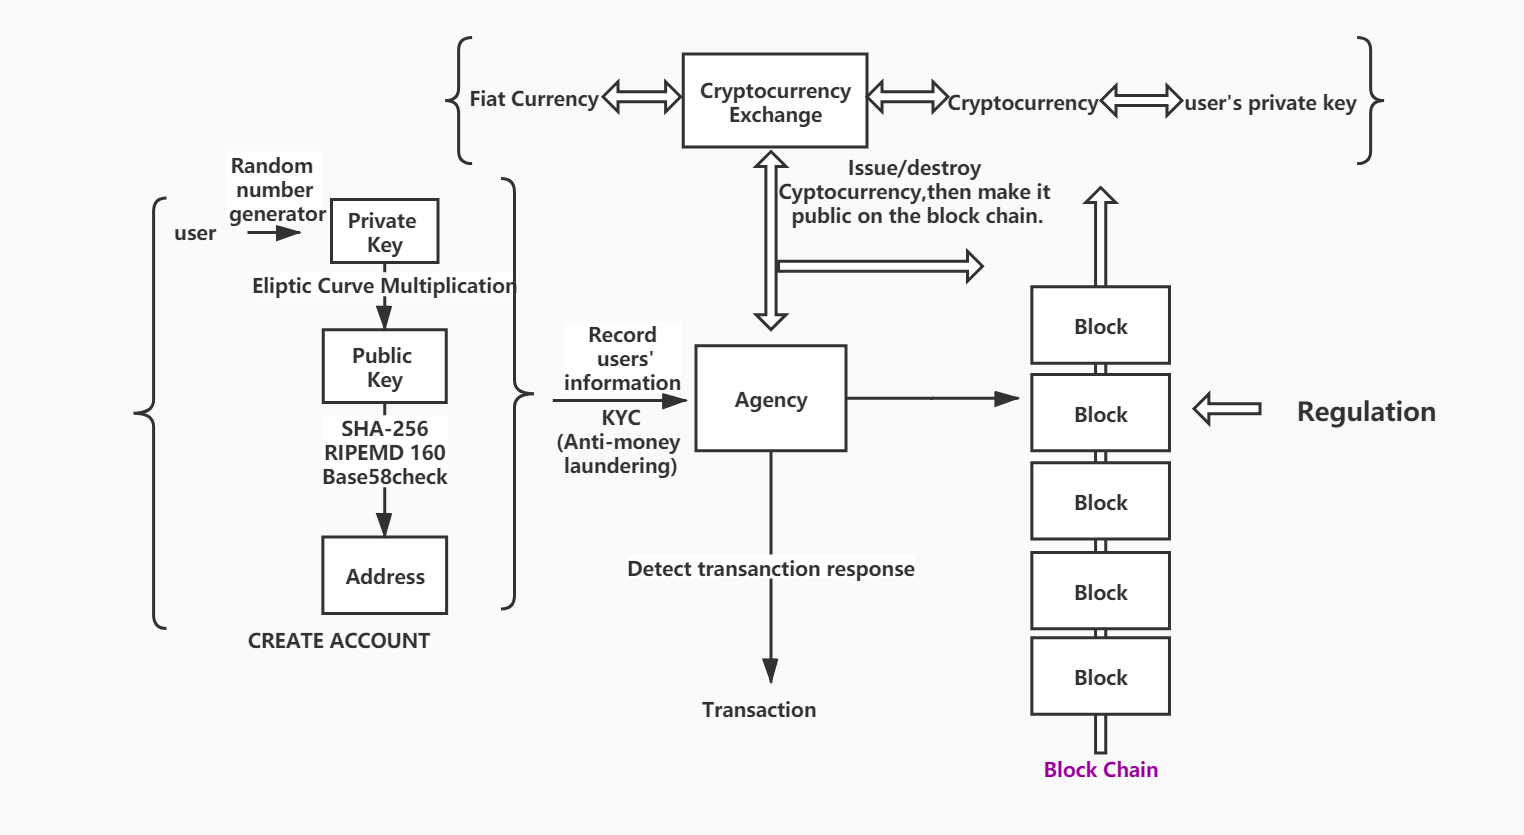
\includegraphics[width=9cm]{Zheng Liu.jpg}
\\
cryptocurrency structure as shown above\cite{zetzsche2019regulating}.

\subsection{Create Account}\label{AA}
Users submit a request. Agency will record users' information to prevent anti-money laundering. Using random number generator to get the private key, then get public key by eliptic curve multiplication.Encrypt the public key by SHA-256\cite{gilbert2003security},RIPEMD 160\cite{dobbertin1996ripemd},Base58check, then we get the user's address.

\subsection{Cryptocurrency Exchange}
Agency works as Cryptocurrency Exchange. It provides the service of exchanging currency. Users can exchange their Fiat Currency like US dollar, Euro, RMB to Crpytocurrency,vice versa.The exchange rate will strictly follow the basket of currencies to ensure the stability of cryptocurrency, strengthen its currency property and reduce speculation bubbles.

Agency also can issue or destroy cryptocurrency based on cryptocurrency exchange to stabilize cryptocurrency value. All the record of issuing and destriying crpytocurrency will be public on the block chain so that anyone can see it on the blockchain\cite{bohme2015bitcoin}.

\subsection{Publish Transaction}
Aency will detect transaction response all the time. It will confirm transaction and get service charge. Then pack account book and make all transactions public on the block chain. All transaction can be traced by users' address. 

\subsection{Regulation}
Account book, transaction, money chain are open to everyone and can not be deleted and modified.

Meanwhile, only the agency can match up the public key used for transaction with certain user. By doing so, we can effectively track illegal  transactions and money laundering.

\section{Agency Encryption Algorithm}
This part is how the agency works and how it connected to Bitcoin. For the reason that currently, Bitcoin is not quite safe, we need to add some management system to make the transaction safer.
\\
\\
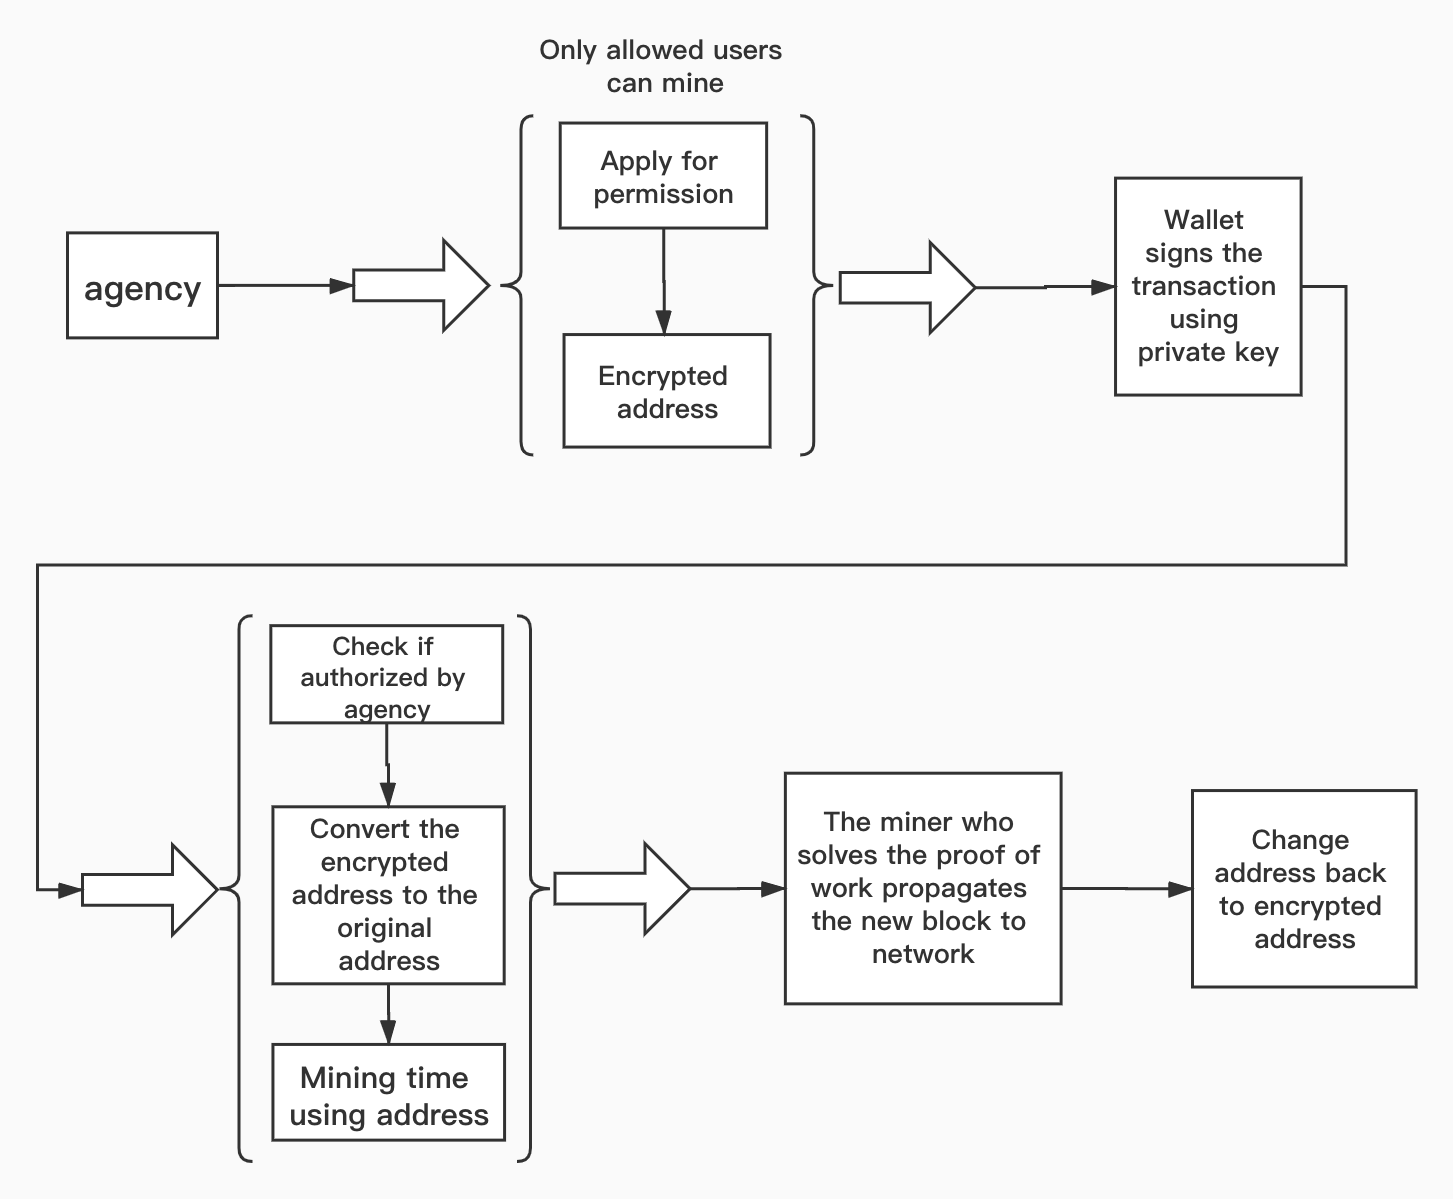
\includegraphics[width=8cm]{xintang He.png}
\\
\\

Use HashMap to store the information of original address, how many bits we added and what address we added. Then determine the user's legitimacy by determining whether the address is 36 bits and the address we get through HashMap is the same as original address.

\subsection{Encrypted Original Address}
Encrypt the original address through add the random(0,1) to its end, and then use a HashMap to memorize the address we add and the length of the address we add, then return the encrypted address.

\subsection{Decode Encrypted Address}
For the reason that we need to use original address to mine, so we need to get the original address. And we can get the original address because we store the information of the address we added by HashMap.

\subsection{Check If The Encrypted Address Is Valid}
If and only if the address we can reach through encrypted address(target) is the same as original address, and the length of target is 36, then we can say this encrypted address is valid\cite{cormen2009introduction}.

\section{Transaction}
The transaction of Bitcoin is very complicated. There are many validation processes involved\cite{moser2013anonymity}. 
\subsection{Get Wallet}
First of all, there will be a random address, and this random address will be transformed to private key with some algorithm. Then we can get a public key from this private key. Wallet address comes from this public key. Wallet address will keep search all transaction in the block.

\\
\\
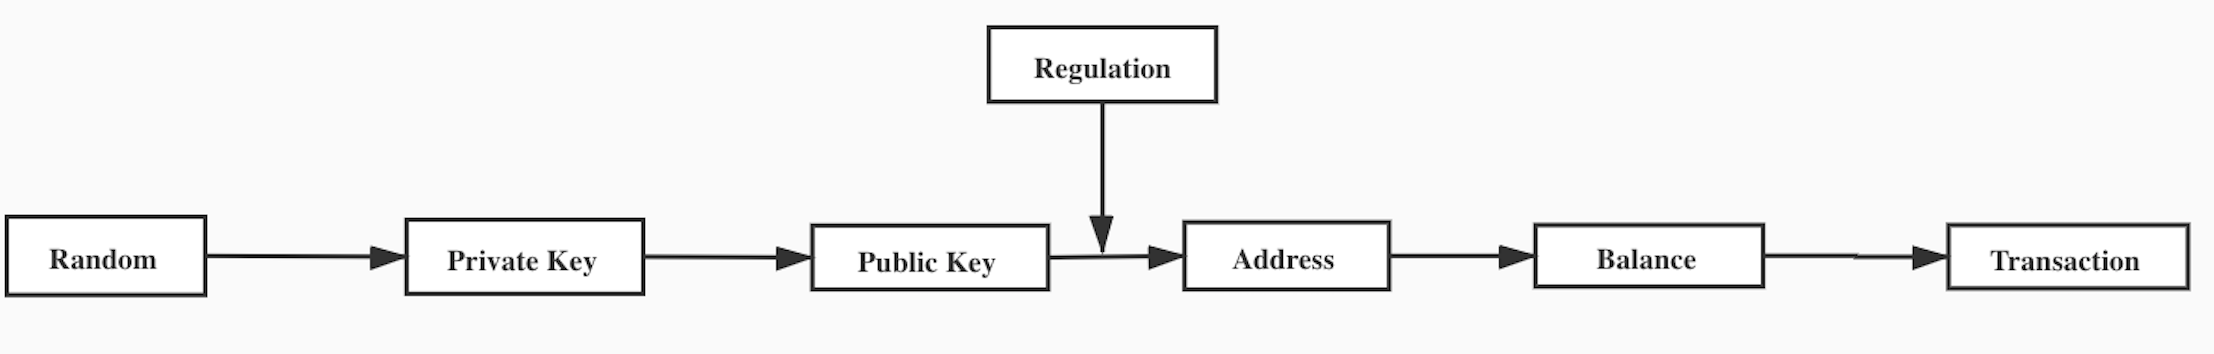
\includegraphics[width=9cm]{likai2.png}
\\
\\

\subsection{Start Transaction}
When someone make a transaction (For example A make a transaction to B), there will be generated an abstract-I by hash algorithm. Then the abstract-I will be encrypted with private key to an autograph. The autograph and public key will be sent to whole block. Block send public key and autograph to some miner. 
\subsection{Validation}
The miner will get public key from A at the same time. Then the miner deciphers the autograph with this public key, and the result is abstract-II. Abstract-II will be contrasted with abstract-I. If these two abstracts are the same, the block will receive an order which said “hey, this transaction is Verified”.
\subsection{Record}
Every transaction record like this processing will be kept in the block which will be checked in all the next deals. And miner can get their bonus when they deal with these validation process. One transaction can only be admitted in the block when all transactions before it is approved. 
\\
\\
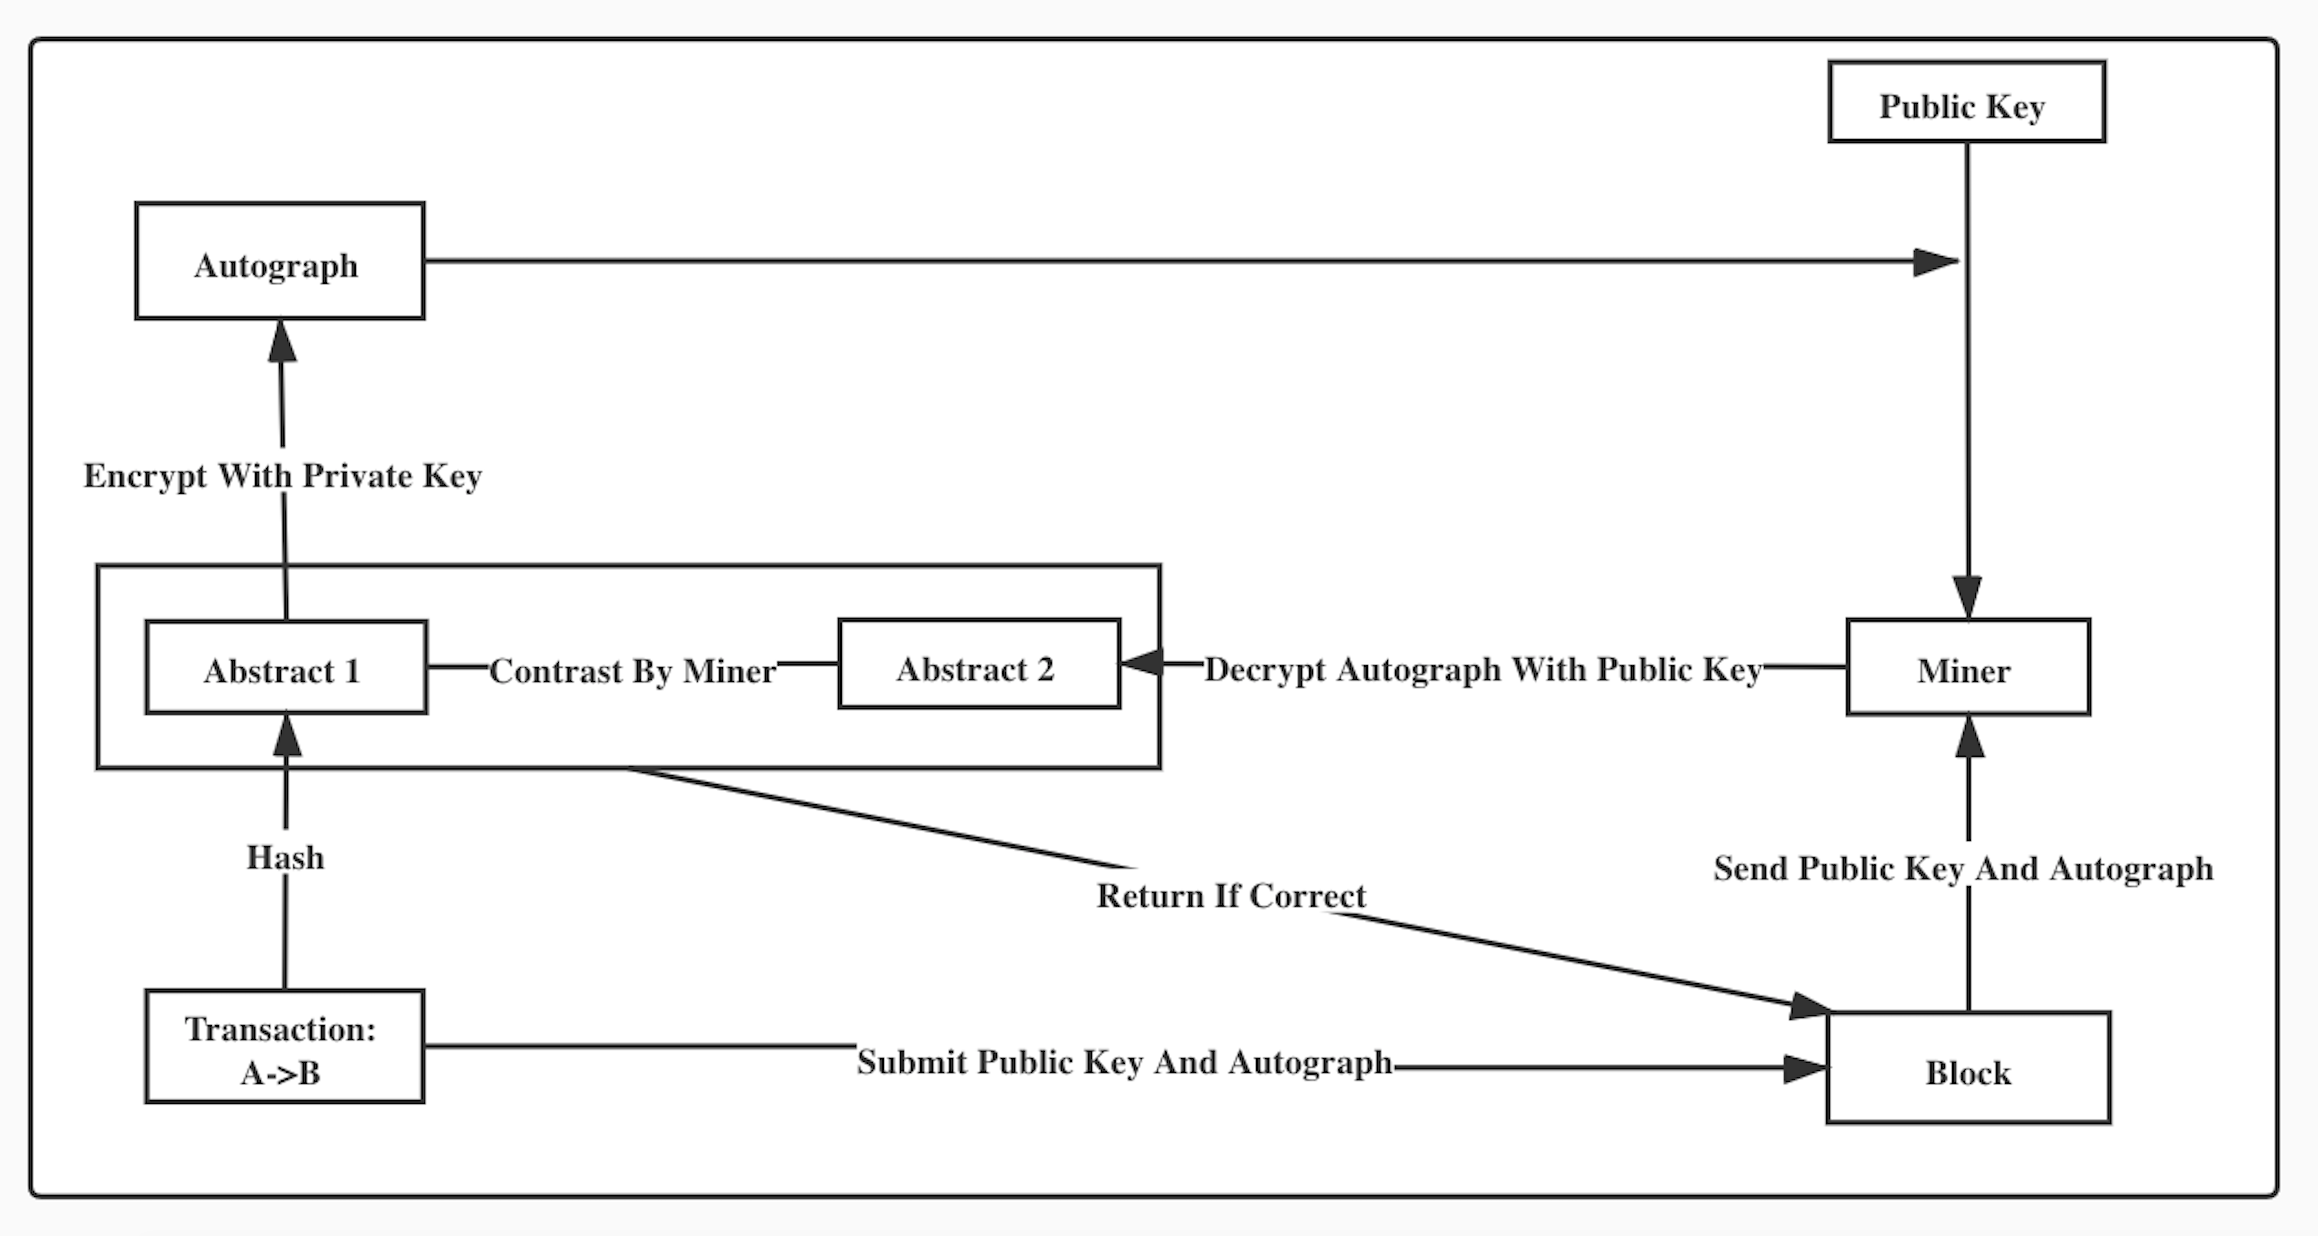
\includegraphics[width = 9cm]{likai1.png}
\\
\\

So, in my opinion, if we want to make the system of Bitcoin run under regulation like Libra but keep its non-centralization. The best way is to find an algorithm that can transform the public key of those who voluntarily accept regulation to a new one.  In order to get the new under-regulation key, you have to submit an application attached with your personal information to the agency and wait for approval and your new key. Those who get a new under-regulation key can do everything with their bitcoin and others may get some restriction.




\section*{Acknowledgment}

Thanks Professor Aftab Ahmad for your guidance during the project. It helps us find the direction and overcome a lot of problems.


\bibliographystyle{./bibliography/IEEEtran}
\bibliography{./bibliography/IEEEabrv,./bibliography/593.bib}

\end{document}
